
\documentclass[12pt]{standalone}
\usepackage{tikz}
%\usetikzlibrary{calc, arrows.meta, decorations.pathreplacing}

\begin{document}

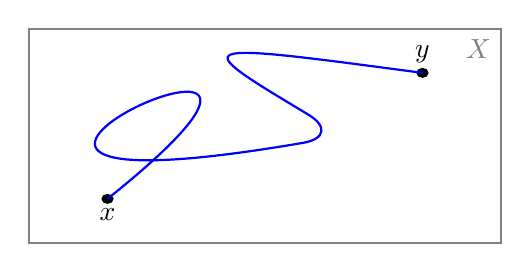
\begin{tikzpicture}[yscale=0.8]
	
	% Draw the topological space X as a rectangle
	\draw[thick, gray, use as bounding box] (0, 0.3) rectangle (6, 3.7) node[anchor=north east] {$X$};
	
	% Define points x and y
	\filldraw (1, 1) circle (2pt) node[anchor=north] {$x$};
	\filldraw (5, 3) circle (2pt) node[anchor=south] {$y$};
	
	% Draw a continuous curve connecting x and y
	\draw[thick, blue, rounded corners=15pt] 
	(1, 1) .. controls (5, 5) and (-3, 0.5) .. (4, 2) .. controls (2, 3.5) .. (5, 3);
	
\end{tikzpicture}


\end{document}

%lwarp%\begin{lateximage}[two points inside a rectangle joined by a continuous path][][width: 50\%;]
